\documentclass[a4paper,11pt,oneside]{scrreprt}
\usepackage[latin1]{inputenc}
\usepackage[english]{babel}
\usepackage{graphicx}
\usepackage{float}
\usepackage{geometry}
\geometry{verbose,a4paper,tmargin=25mm,bmargin=25mm,lmargin=10mm,rmargin=10mm}
\usepackage{paralist}

\usepackage{paracol}

\usepackage{todonotes}

\usepackage{listings}
\lstset{language=Java,
	tabsize=2,
	showspaces=false,
	showtabs=false,
	breaklines=true,
	showstringspaces=false,
	breakatwhitespace=true,
	commentstyle=\color{pgreen},
	keywordstyle=\color{pblue},
	stringstyle=\color{pred},
	basicstyle=\footnotesize\ttfamily,
	moredelim=[il][\textcolor{pgrey}]{$$},
	moredelim=[is][\textcolor{pgrey}]{\%\%}{\%\%}
}

\usepackage{tikz}
\usetikzlibrary{calc,patterns,angles,quotes}

\usepackage{caption}
\usepackage{subcaption}
\usepackage{tabularx} % in the preamble

\usepackage{pdfpages}

\usepackage{indentfirst} % for always indenting the first paragraphs

\begin{document}


\begin{center}
	Submitted by Group 18
	
	\bigskip
	
	\begin{tabular}{c}
	Group Members: \\
	CETIN, Ulfet (391819); GRUCZKA, FILIP (413279);	LIPINSKI, Bartosz (413177) \\
	\end{tabular}

	\bigskip
	
	DIS1 WS 19/20 - Project Milestone I\\
	Problem Definition
	
	%	(ordered on lastname basis)
\end{center}
\vspace{0cm}

\begingroup
\let\clearpage\relax
	\chapter{The Problem \#1: Shopping for Kitchen}
\endgroup
	
		\indent Organizing a healthy diet via cooking at home is a chore in and out of itself with all its needs such as keeping refrigerator organized, keeping track of the best before dates, and coming up with recipes that can be achievable with what is already in hand.\\
		
		In order to see what our user group experience, we hold user interviews to observe them. Before starting, they were informed about the nature of the questions and that they have to answer as their heart desires. Also their permission is asked to use the information provided by them in this assignments. The questions that we are provided are asked on one-on-one interviews that are held in isolation, two in their kitchen, three in other places. While asking questions, no leads or hints has been provided, and when asked, they were replied with the statement that they can answer as they desire, as long as they respect the question body.\\
		
		Also, the some of the sources that have been read:
			\begin{compactitem}
				\item http://blog.chefsplate.com/10-common-cooking-problems/\\
				more of a compilation of cooking problems (yet seen to be correlated with interviewee \#3 on missing ingredients)
				
				\item https://www.helpguide.org/articles/healthy-eating/cooking-at-home.htm\\
				guide on cooking at home, with stated common obstacles
				
				
			\end{compactitem}
		
		\section{Interview Questions}
			
			\begin{compactitem}
				\item How do you describe yourself in the kitchen? More like a cook or an eater, basically?
				\item How much time do you spend in the kitchen?
				\item All the time that you spend in the kitchen, and imagining yourself in your kitchen, what chores do you remember you are doing?
				\item Which ones of those chores you find boring? (also, please state the ones you find enjoyable). And why?
				\item Among those, which dreads you the most? And why?
			\end{compactitem}
	
	\section{Answers from the Interviewees}
	
		\begin{compactitem}
			\item interviewee \#1	
				\begin{compactitem}
					\item Information about the interviewer: \\
					age 27, Caucasian female, student in RWTH in Data Science M.Sc., married, living in a household of two with her husband\\
					
					\item Answers summed up from the interviewee:
						\begin{compactenum}
							\item More of a cook, can be considered as fifty-fifty with the husband
							\item at least once in a day, more likely twice including the breakfast, total of around 2 hours
							\item thinking about what to cook in order not to fall into the cycle of eating the same things over a long time (similar with husband), playing the guessing game to see what `we` can cook with the husband, work-distribution (stated they own a dishwasher), cutting the ingredients in shape, actually cooking the food
							\item not finding any of the chores in the kitchen boring (other than some dishes that has to be hand-washed)
							\item thinking what to cook, although not dreading the interviewee, sometimes frustrates, where it is hard to come up with something new
						\end{compactenum}
					
					
				\end{compactitem}
			
			\bigskip
			
			\item interviewee \#2
			\begin{compactitem}
				\item Information about the interviewer: \\
				age 24, Caucasian female, student in RWTH in Industrial Engineering M.Sc., single, living in a shared flat with 2 other people
				
				\item Answers summed up from the interviewee:
				\begin{compactenum}
					\item both cook and eater, as she cooks alone mostly
					\item once in a day, less than an hour
					\item feels like it has been a century in the kitchen: deciding, getting the ingredients out, preparing, staying alert near the topf, serving, cleaning afterwards
					\item always eating pasta, although not changing it. (what she likes: trying new recipes, although seldom)
					\item not eating healthy, not liking to spend time in kitchen although wanting to. (when asked why, she spit out that she does not have the skills and the necessary knowledge to cook other things)
				\end{compactenum}
				
				
			\end{compactitem}
		
			\bigskip
			
			\item interviewee \#3
			\begin{compactitem}
				\item Information about the interviewer: \\
				age 28, Caucasian male, student in RWTH working on a Phd (field not specified), married, living in a household of two with his wife\\
				
				\item Answers summed up from the interviewee:
				\begin{compactenum}
					\item states himself to be `helper`, as cooking with the wife
					\item around 3 hours
					\item discussing what to eat, sometimes going out to buy the lacking ingredients of a specific recipe, filling the dishwasher and emptying it, giving a helping hand to the wife on what duty calls
					\item not knowing what to eat for each afternoon, and trying to come up with ideas on what to eat
					\item finding a food idea that her wife accepts
				\end{compactenum}
				
				
			\end{compactitem}
		\end{compactitem}
		
	\section{Problem Statement}
		Out of five people we interviewed, we analyzed all and we put down the three of them we find interesting. The following is the problem statement after analyzing all the five cases, which we `might` aim to solve:\\
		
	
		\begin{tabularx}{\textwidth}{|X|}
	
			\hline
				\textbf{Problem Statement:}\\
				
				People spending too much time deciding on what to buy for their refrigerators \& what to cook using the ingredients in the said refrigerator. Moreover, they get frustrated or bored because they spend so much time \& got a little gain from their spent time and effort.\\
				
			\hline
			
		\end{tabularx}



%\begin{figure}[H]
%	\centering
%	\begin{subfigure}{.5\textwidth}
%		\centering
%		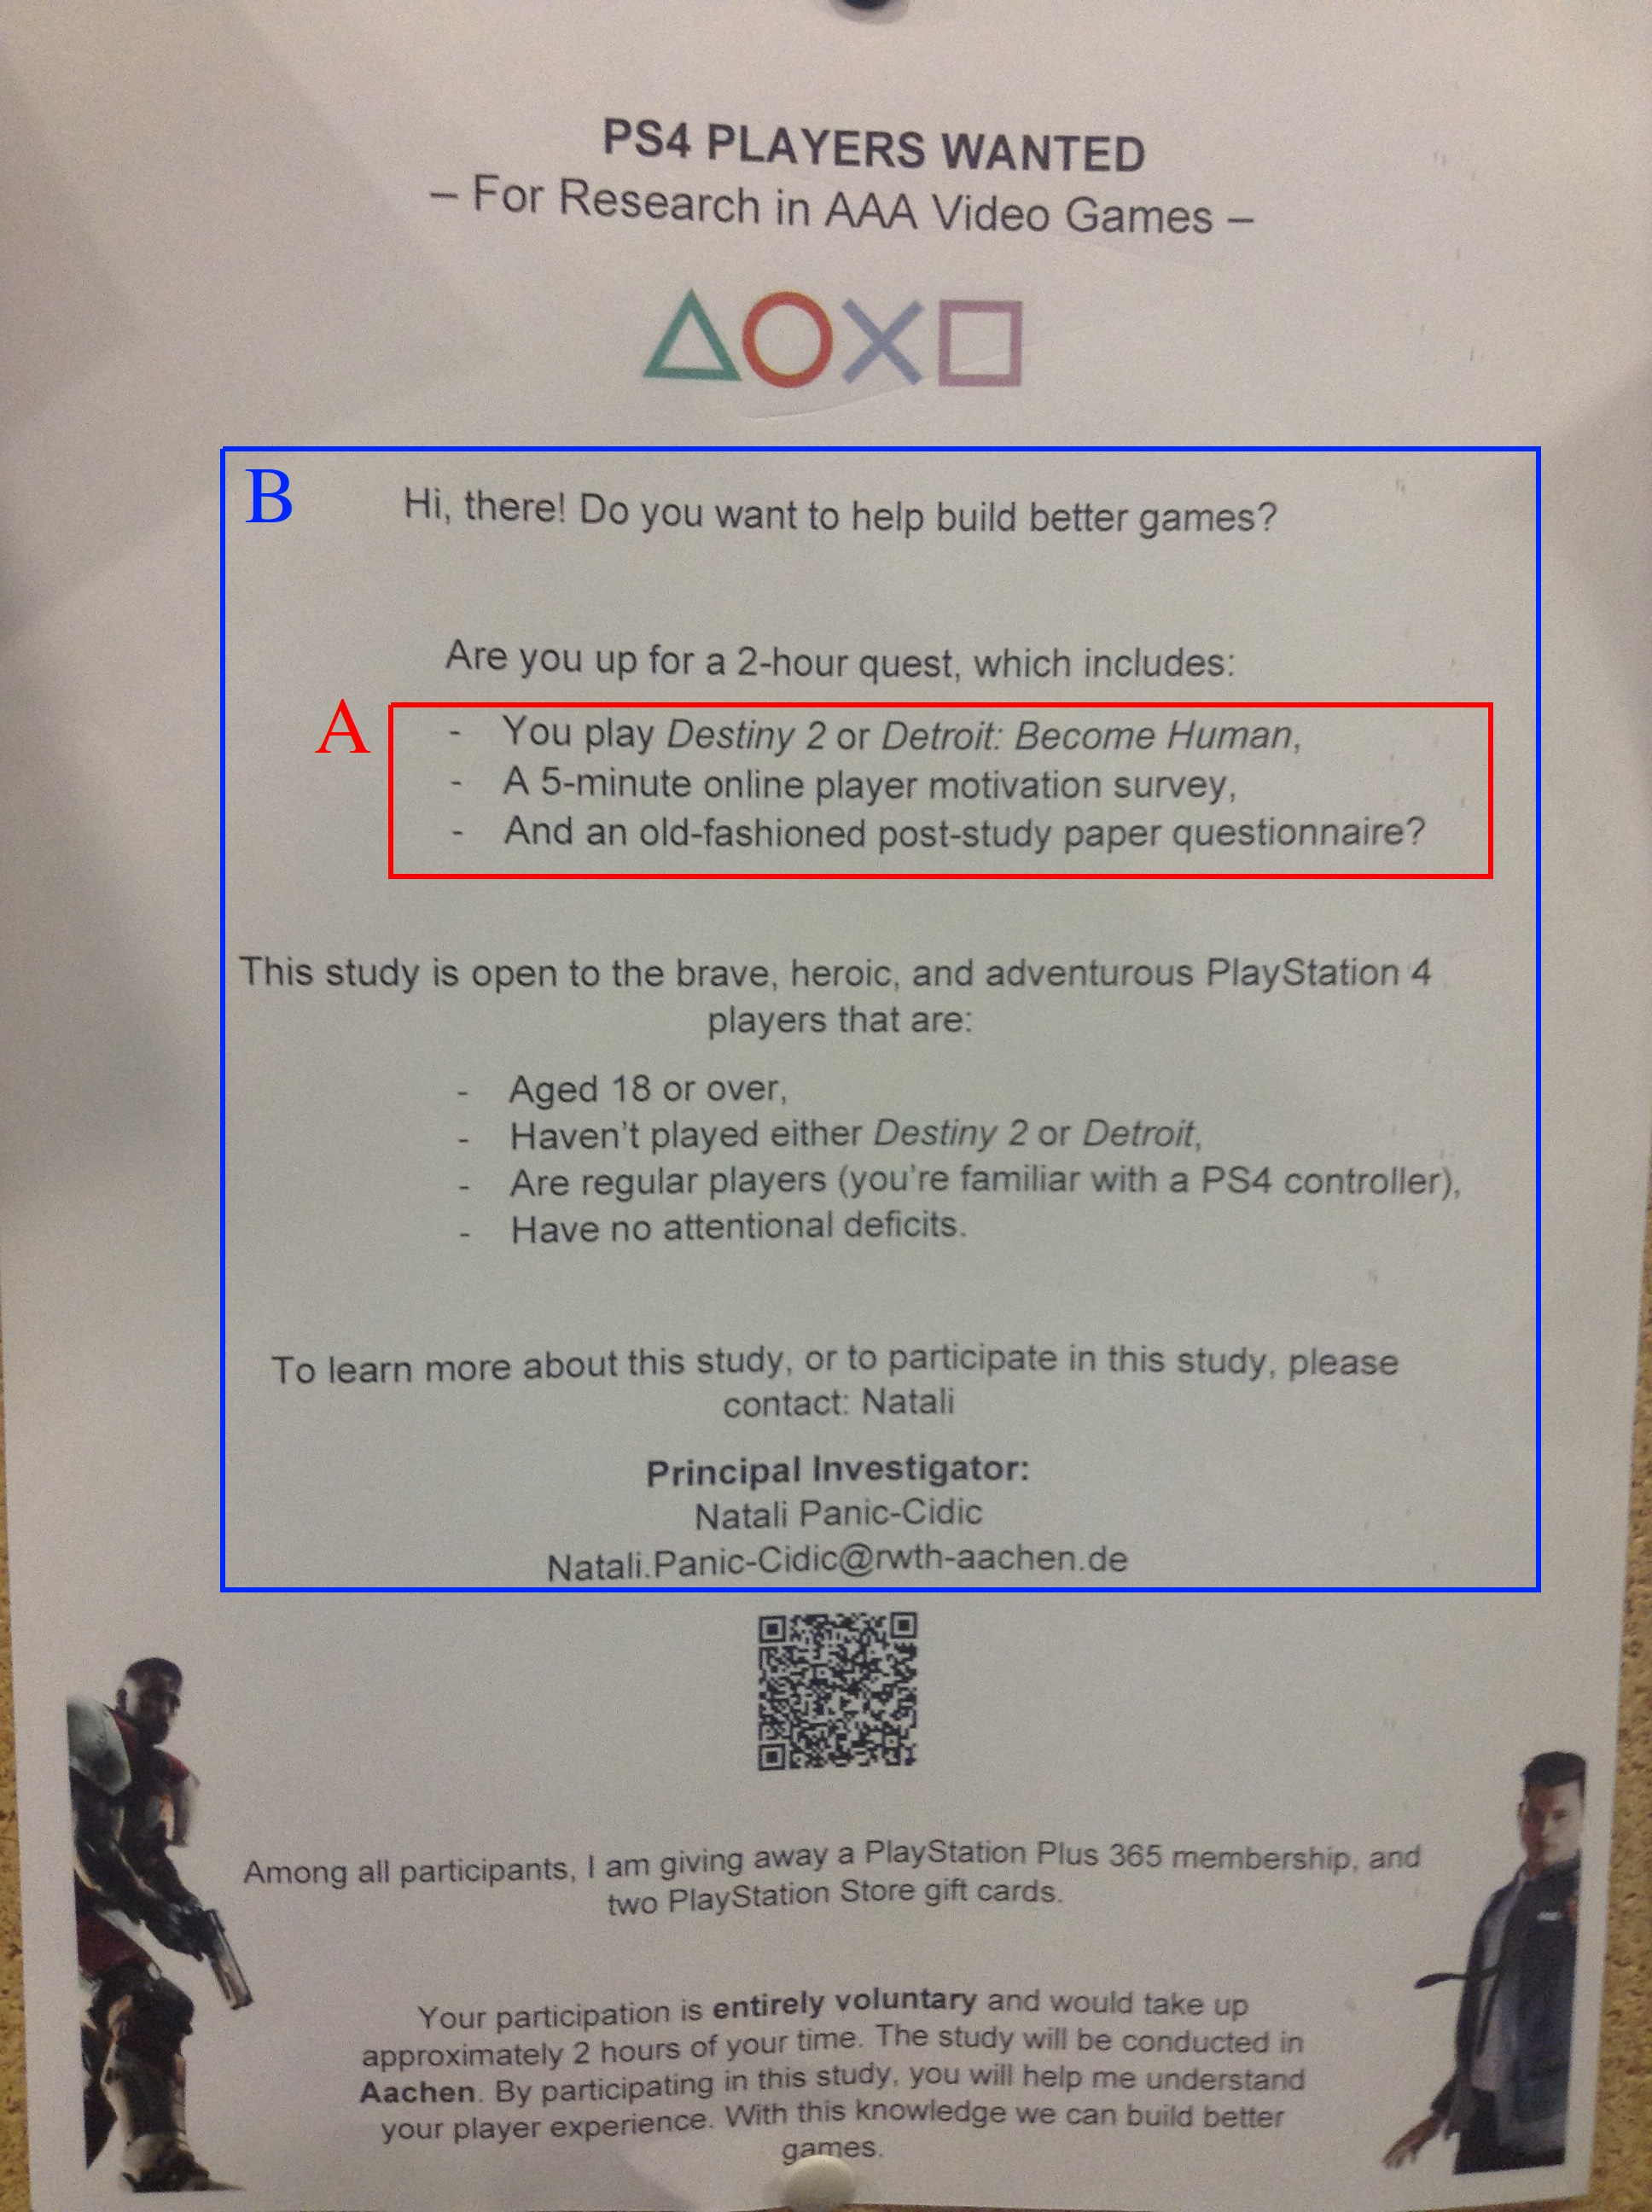
\includegraphics[clip, trim=0cm 0cm 0cm 0cm, scale=0.12]{./images/recruitment2.jpeg}
%		\caption{PS4 Player Ad}
%%		\label{fig:sub1}
%	\end{subfigure}%
%	\begin{subfigure}{.5\textwidth}
%		\centering
%		
\includegraphics[clip, trim=0cm 0cm 0cm 0cm, scale=0.53]{./images/proximity.jpg}
%		\caption{Event Schedule}
%%		\label{fig:sub2}
%	\end{subfigure}
%\end{figure}

%\begin{tabularx}{\textwidth}{|X|}
%	\hline
%		\textbf{Violations of Visual Design Principles}
%		\\
%	\hline
%		\textbf{Violation \#1:} Contrast (PS4 Player Ad)\\
%		Picture: \textbf{PS4 Player Ad:B}\\
%		
%		\\
%		\textbf{Describe Violation:} Nearly no contrast, so many information with no distinction between nearly any text (titles have no contrast to the texts under them)
%		
%		
%		\\
%		\textbf{Why Bad?:} Makes it hard to distinguish between parts, and makes it hard to digest all the text. Assuming it has bold or larger subheaders (such as "Are you up for a 2-hour quest, which includes :" and "This study is open to brave, heroic, adventurous PS4 players that are:"), it would have been easier to understand the bill at the first glance. Although whitespace usage is not bad, he current form leads to more mental work distinguishing parts.
%		
%	\\
%	\hline
%	
%		\textbf{Violation \#2:} Repetition (PS4 Player Ad)\\
%		Picture: \textbf{PS4 Player Ad:B}
%		
%		\\
%		\textbf{Describe Violation:} There is no consistent good repetition in the design. Aside from the same font size being used nearly everywhere, no part of the text and layout has been stepping forward to make a change in the view. This leads to dull-looking design. Note that there are tiny differences in the visual that steps forward like the main header "PS4 Players Wanted", and name of the investigator being bold, and two more; but those are few, thus, the style is repetitive in a negative sense, this repetitiveness does not help the user at all. 
%		
%		\\
%		\textbf{Why Bad?:} User wants positive repetitiveness, and wants to know what to look at, how to continue reading text; in general, a good flow of style together with objects aligned well, like the CV example in the slides. In this, we have no such thing, the user is not 'guided' by the style that does not convey the idea of where to look. This is unstructured, or let's say repetitive in a bad manner that nothing gives out user any clue on what is important, where is the keypoints and so on.
%		
%	\\
%	\hline	
%	
%		\textbf{Violation \#3:} Proximity (PS4 Player Ad)\\
%		Picture: \textbf{PS4 Player Ad:A}
%		
%		\\
%		\textbf{Describe Violation:} The list points(dashes) and the correspongding list items(texts) in the given bill have so much space in between them that them seem separate.
%		
%		\\
%		\textbf{Why Bad?:} The list points and the list items observed as being separate does not help user digest them as coupled together, it is the other way, them seem separate. This leads to reading and observing difficulty, as they are not in their proximity, that is, not close enough.
%		
%		\\
%		\hline	
%	
%\end{tabularx}\\

\end{document}}
